\chapter{評価}

\label{evaluation}
本研究では、本システムを利用することでポーズが改善できるかの検証、また、既存の練習方法である鏡を用いた練習との比較を行うため、
練習前と練習後、練習から24時間後のポーズの比較と、各ポーズにおけるシステム利用群と鏡利用群の比較を行った。
\section{評価内容}
  今回はシステムでのフィードバックでは両肘、両肩の角度についてフィードバックを行なっていたため、評価の際も同様に両肘、両肩の角度について評価を行った。


  肩の角度 \(\theta_{\text{肩}}\) は、上腕の単位ベクトル \(\vec{u}\) と両肩を結ぶ線の単位ベクトル \(\vec{w}\) を用いて計算することができる。この角度は、以下の式で定義される:

  \[
  \theta_{\text{肩}} = \cos\left( \frac{\vec{u} \cdot \vec{w}}{\|\vec{u}\| \|\vec{w}\|} \right) \times \frac{180}{\pi}
  \]


  同様に、肘の角度 \(\theta_{\text{肘}}\) は、前腕の単位ベクトル \(\vec{v}\) と上腕の単位ベクトル \(\vec{u}\) を使用して次のように計算される:

  \[
  \theta_{\text{肘}} = \cos\left( \frac{\vec{v} \cdot \vec{u}}{\|\vec{v}\| \|\vec{u}\|} \right) \times \frac{180}{\pi}
  \]

\section{測定方法}
  練習前、練習後、24時間後に写真を撮影し、それをMediapipe Poseを用い、ポーズを解析し角度を測定した。
  今回はMediapipe PoseでもBlazePose GHUM Heavyモデルを用いた。BlazePose GHUM Heavyモデルは表 \ref{tab:pose-estimation-quality} に示す通り同じBlazePose GHUMのモデルや、AlphaPose ResNet50、Apple Visionと比較しても様々なアクティビティにおいて精度が高いことが報告されている。
  この評価で用いられているPCK@0.2とは、人体の各部位の予測点と実際の点の距離が、人体の幅の20\%以内にあるかどうかを判定する指標である。\cite{PCK} また、利用者の属する地域別の精度は 図\ref{fig:Model-Accuracy-by-Race} に示す。今回の被験者の所属する日本は、Eastern Asiaに属するが、Eastern Asiaでの精度は今回利用するHeavyモデルではPDJという手法で92.6\%となっている。PDJはPCK@0.2と同義である。

  \begin{table}[ht]
    \centering
    \caption{様々なアクティビティにおける様々なモデルのPCK@0.2の比較 \cite{pose-estimation-quality}}
    \begin{tabular}{|l|c|c|c|}
    \hline
    \textbf{Method} & \textbf{Yoga} & \textbf{Dance} & \textbf{HIIT} \\
                    & PCK@0.2       & PCK@0.2        & PCK@0.2       \\ 
    \hline
    BlazePose GHUM Heavy                                                      & \textbf{96.4} & \textbf{97.2} & \textbf{97.5} \\
    BlazePose GHUM Full                                                       & \textbf{95.5} & \textbf{96.3} & \textbf{95.7} \\
    BlazePose GHUM Lite                                                       & \textbf{90.2} & \textbf{92.5} & \textbf{93.5} \\
    \href{https://github.com/MVIG-SJTU/AlphaPose}{AlphaPose ResNet50}         & \textbf{96.0} & \textbf{95.5} & \textbf{96.0} \\
    \href{https://developer.apple.com/documentation/vision/detecting_human_body_poses_in_images}{Apple Vision} & \textbf{82.7} & \textbf{91.4} & \textbf{88.6} \\
    \hline
    \end{tabular}
    \label{tab:pose-estimation-quality}
  \end{table}
    
  \begin{figure}[H]
    \begin{center}
    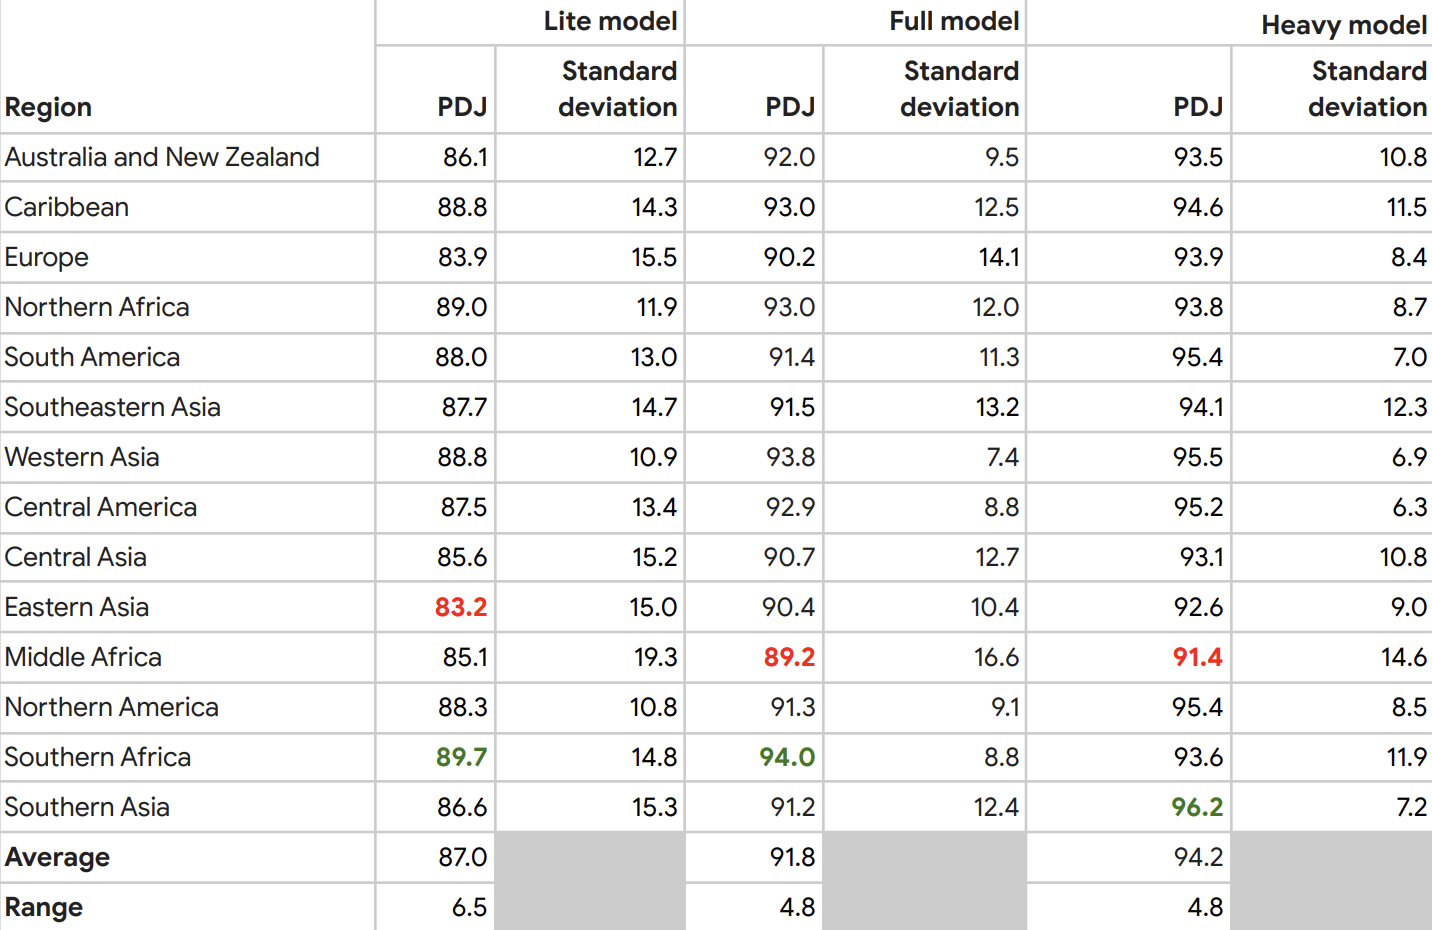
\includegraphics[width=12cm]{figures/Model_Accuracy_by_Race.png}
    \caption{様々な骨格推定モデルの地域別精度 \cite{Model-Accuracy-by-Race}}
    \label{fig:Model-Accuracy-by-Race}
    \end{center}
  \end{figure}

\section{検定手法}
  本研究の実験では被験者が少ないため、ノンパラメトリック検定を用いて検定を行った。
  同一被験者の練習後、24時間後と練習前の理想のポーズの角度の差の検定は、ウィルコクソンの符号付き順位和検定を用いた。
  また、システム利用群と鏡利用群の比較は、ウィルコクソンの順位和検定を用いた。有意水準は0.05とした。
\section{結果}
  本研究では練習で改善されたかどうかを評価したいため、練習前、練習後、24時間後のポーズの角度と理想とするポーズ(システムとしてさせたいポーズ)の両肘両肩の角度の差の平均 \(\bar{\theta}_{\text{angle\_dif}}\)を利用して評価する。
  それぞれの関節を右肘(RE)、左肘(LE)、右肩(RS)、左肩(LS)とし、以下のように定義した。

  \[
    \bar{\theta}_{\text{angle\_dif}} = \frac{1}{4} \sum_{i \in \{\text{RE, LE, RS, LS}\}} |\theta_{i, \text{Actual}} - \theta_{i, \text{Ideal}}|
  \]

  \subsection{練習前後、24時間後の比較}
    ここではシステムを利用して練習した群と鏡を利用して練習した群それぞれの練習前後、24時間後のポーズの理想の角度との差の結果を示す。
    \subsubsection{システム利用群の比較}
      図\ref{fig:pose1_system}にpose1に対してシステムを利用した群の練習前後、24時間後の結果と理想の角度との差の平均\(\bar{\theta}_{\text{angle\_dif}}\)の推移を示す。


      7名のうち、5名の被験者が練習直後は練習前よりポーズが改善されていることがわかる。しかしながら、24時間後では練習前より改善されている被験者は1名のみであった。
      検定の結果では練習後と練習前の差は有意性を示すことができず(p=0.8782)、24時間後と練習前の差も統計的に有意性を示すことができなかった(p=0.4674)。表\ref{table:pose1_system_p_value}

      \begin{figure}[H]
        \begin{center}
        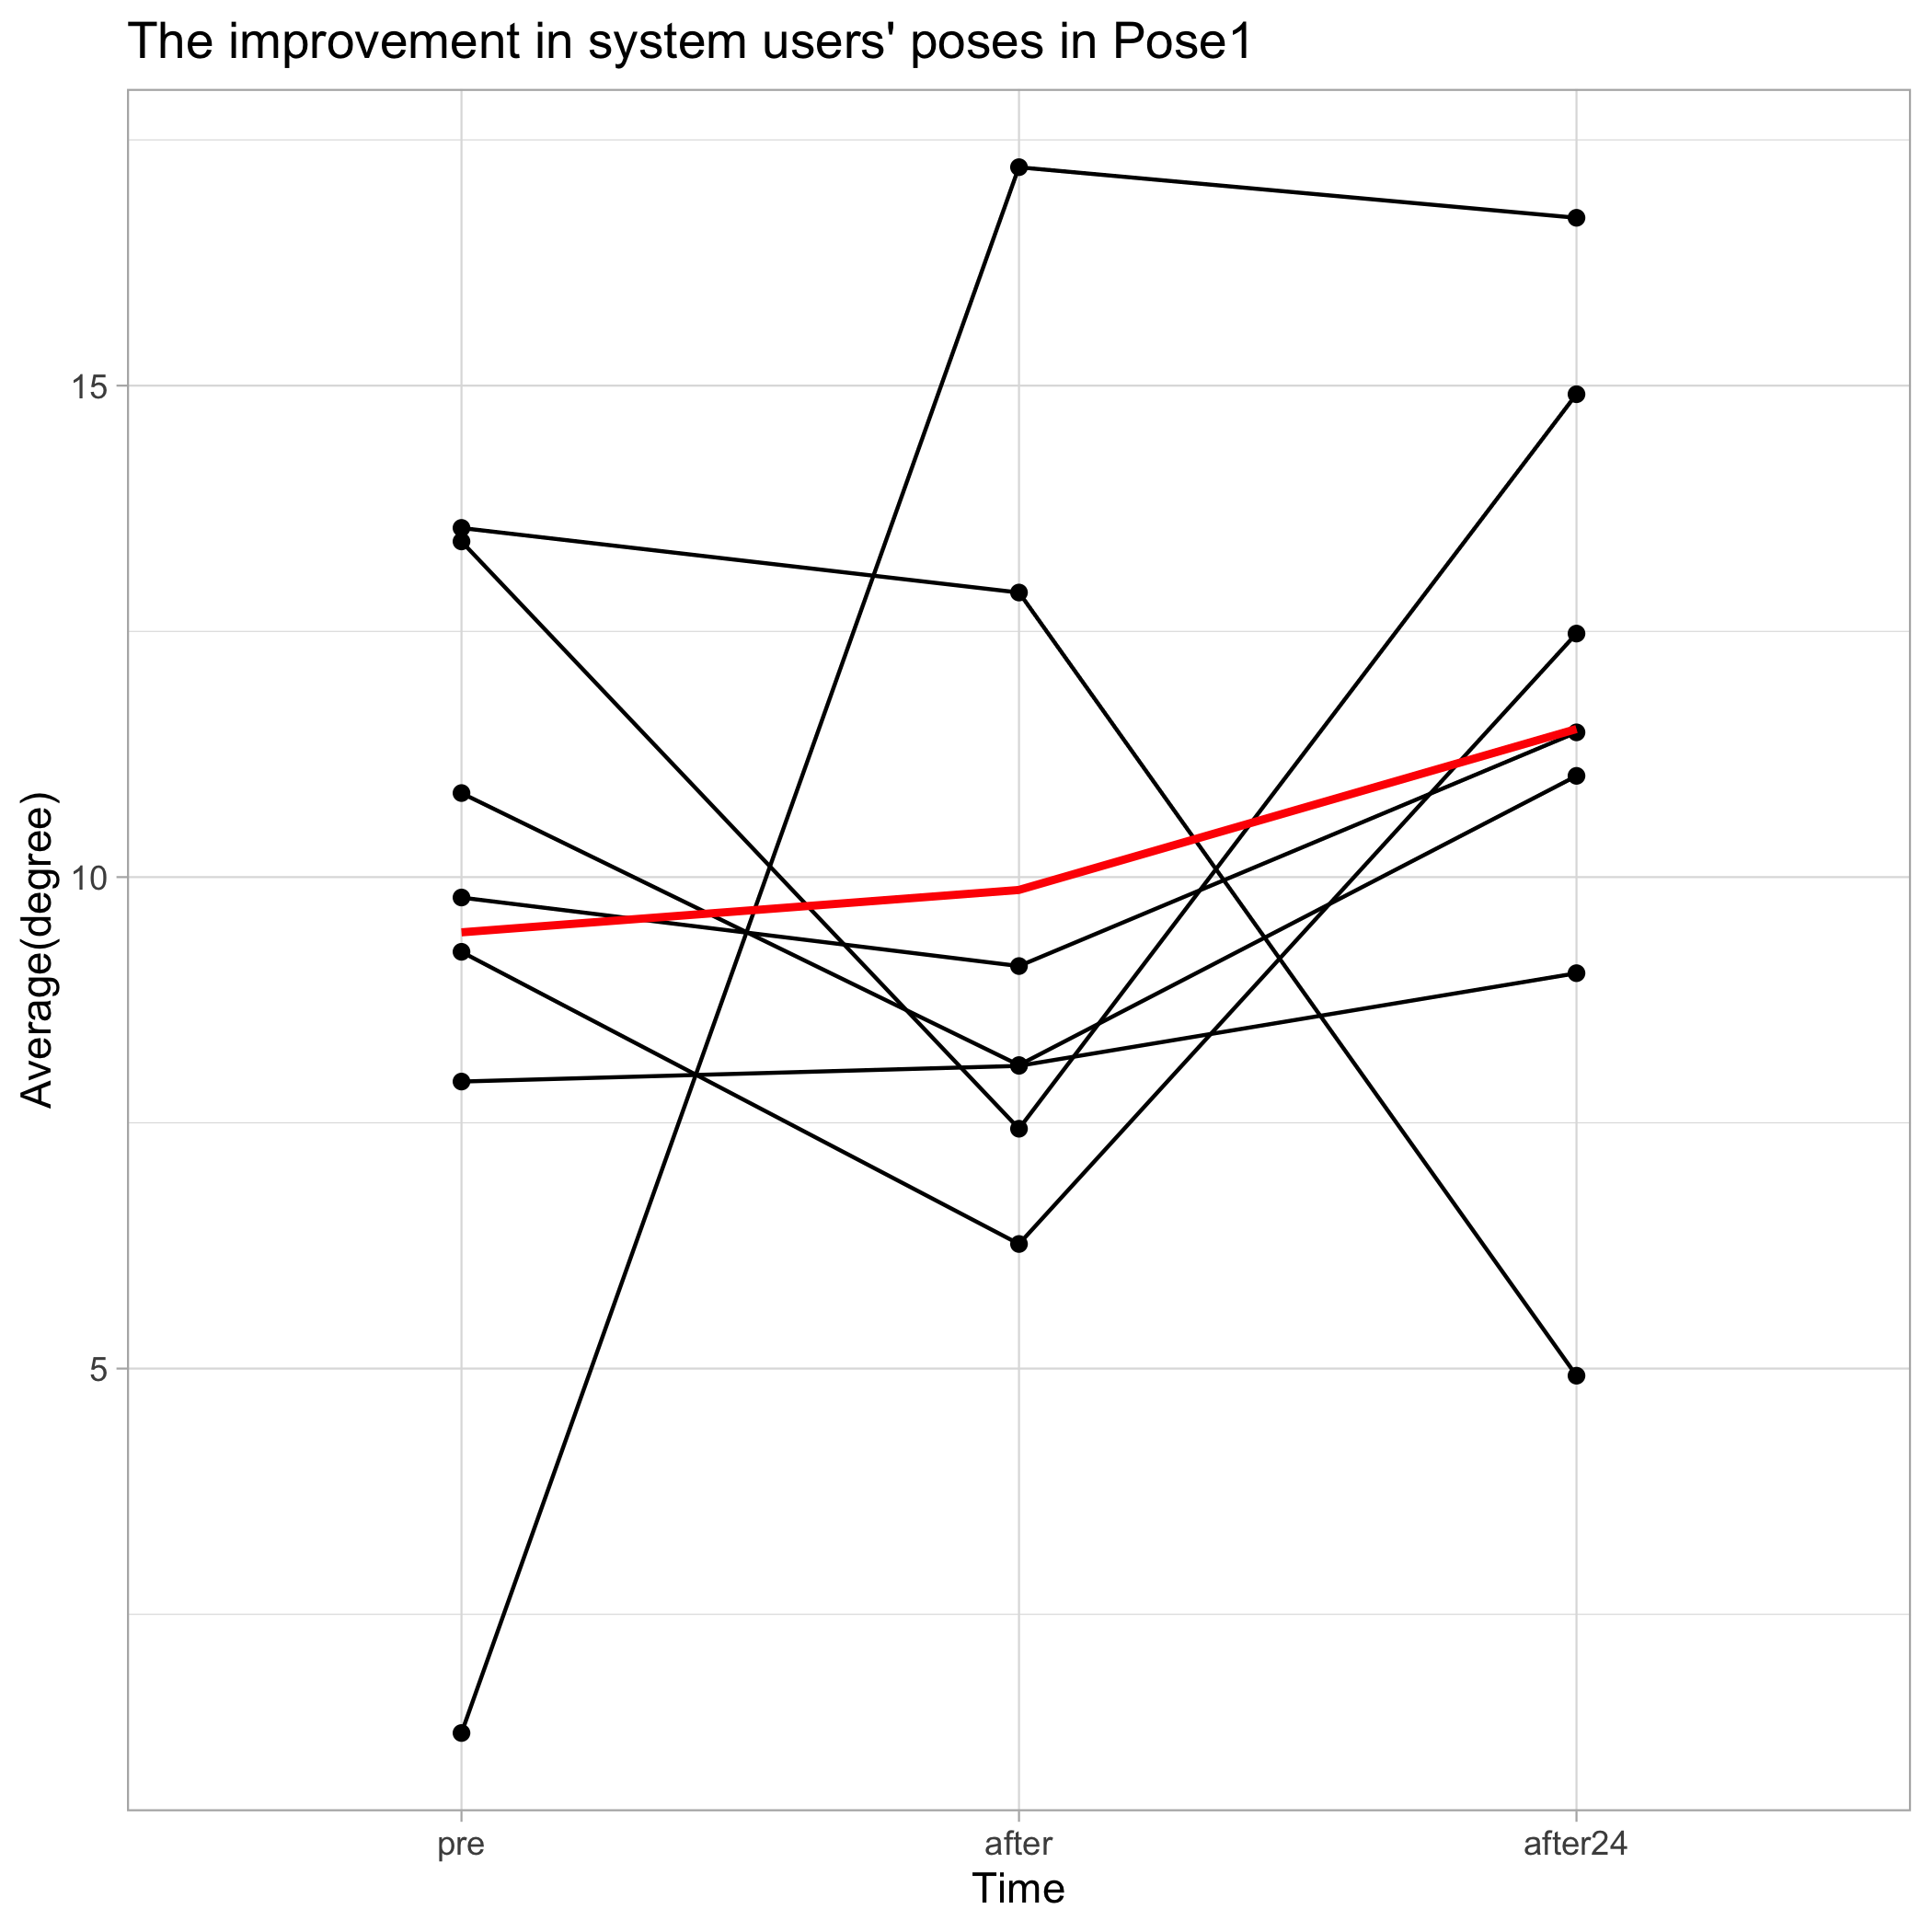
\includegraphics[width=9cm]{figures/pose1_system_true_graph.png}
        \caption{システム利用群のpose1の結果}
        \label{fig:pose1_system}
        \end{center}
      \end{figure}

      \begin{table}[h]
        \centering
        \caption{pose1における練習後、練習から24時間後と練習前の比較}
        \begin{tabular}{lcr}
        \hline
        \textbf{比較対象} & \textbf{p-value} & \textbf{MD} \\ \hline
        練習後-練習前 & 0.8782 & 0.4314286 \\ \hline
        24時間後-練習前 & 0.4674 & 2.068929 \\ \hline
        \end{tabular}
        \label{table:pose1_system_p_value}
        \end{table}

        図\ref{fig:pose2_system}にpose2に対してシステムを利用した群の練習前後、24時間後の結果と理想の角度との差の平均\(\bar{\theta}_{\text{angle\_dif}}\)の推移を示す。


      7名のうち、5名の被験者が練習直後は練習前よりポーズが改善されていることがわかる。しかしながら、24時間後では練習前より改善されている被験者は3名のみであった。
      検定の結果では練習後と練習前の差は有意性を示すことができず(p=0.07812)、24時間後と練習前の差も統計的に有意性を示すことができなかった(p=0.8125)。表\ref{table:pose2_system_p_value}
      \begin{figure}[H]
        \begin{center}
        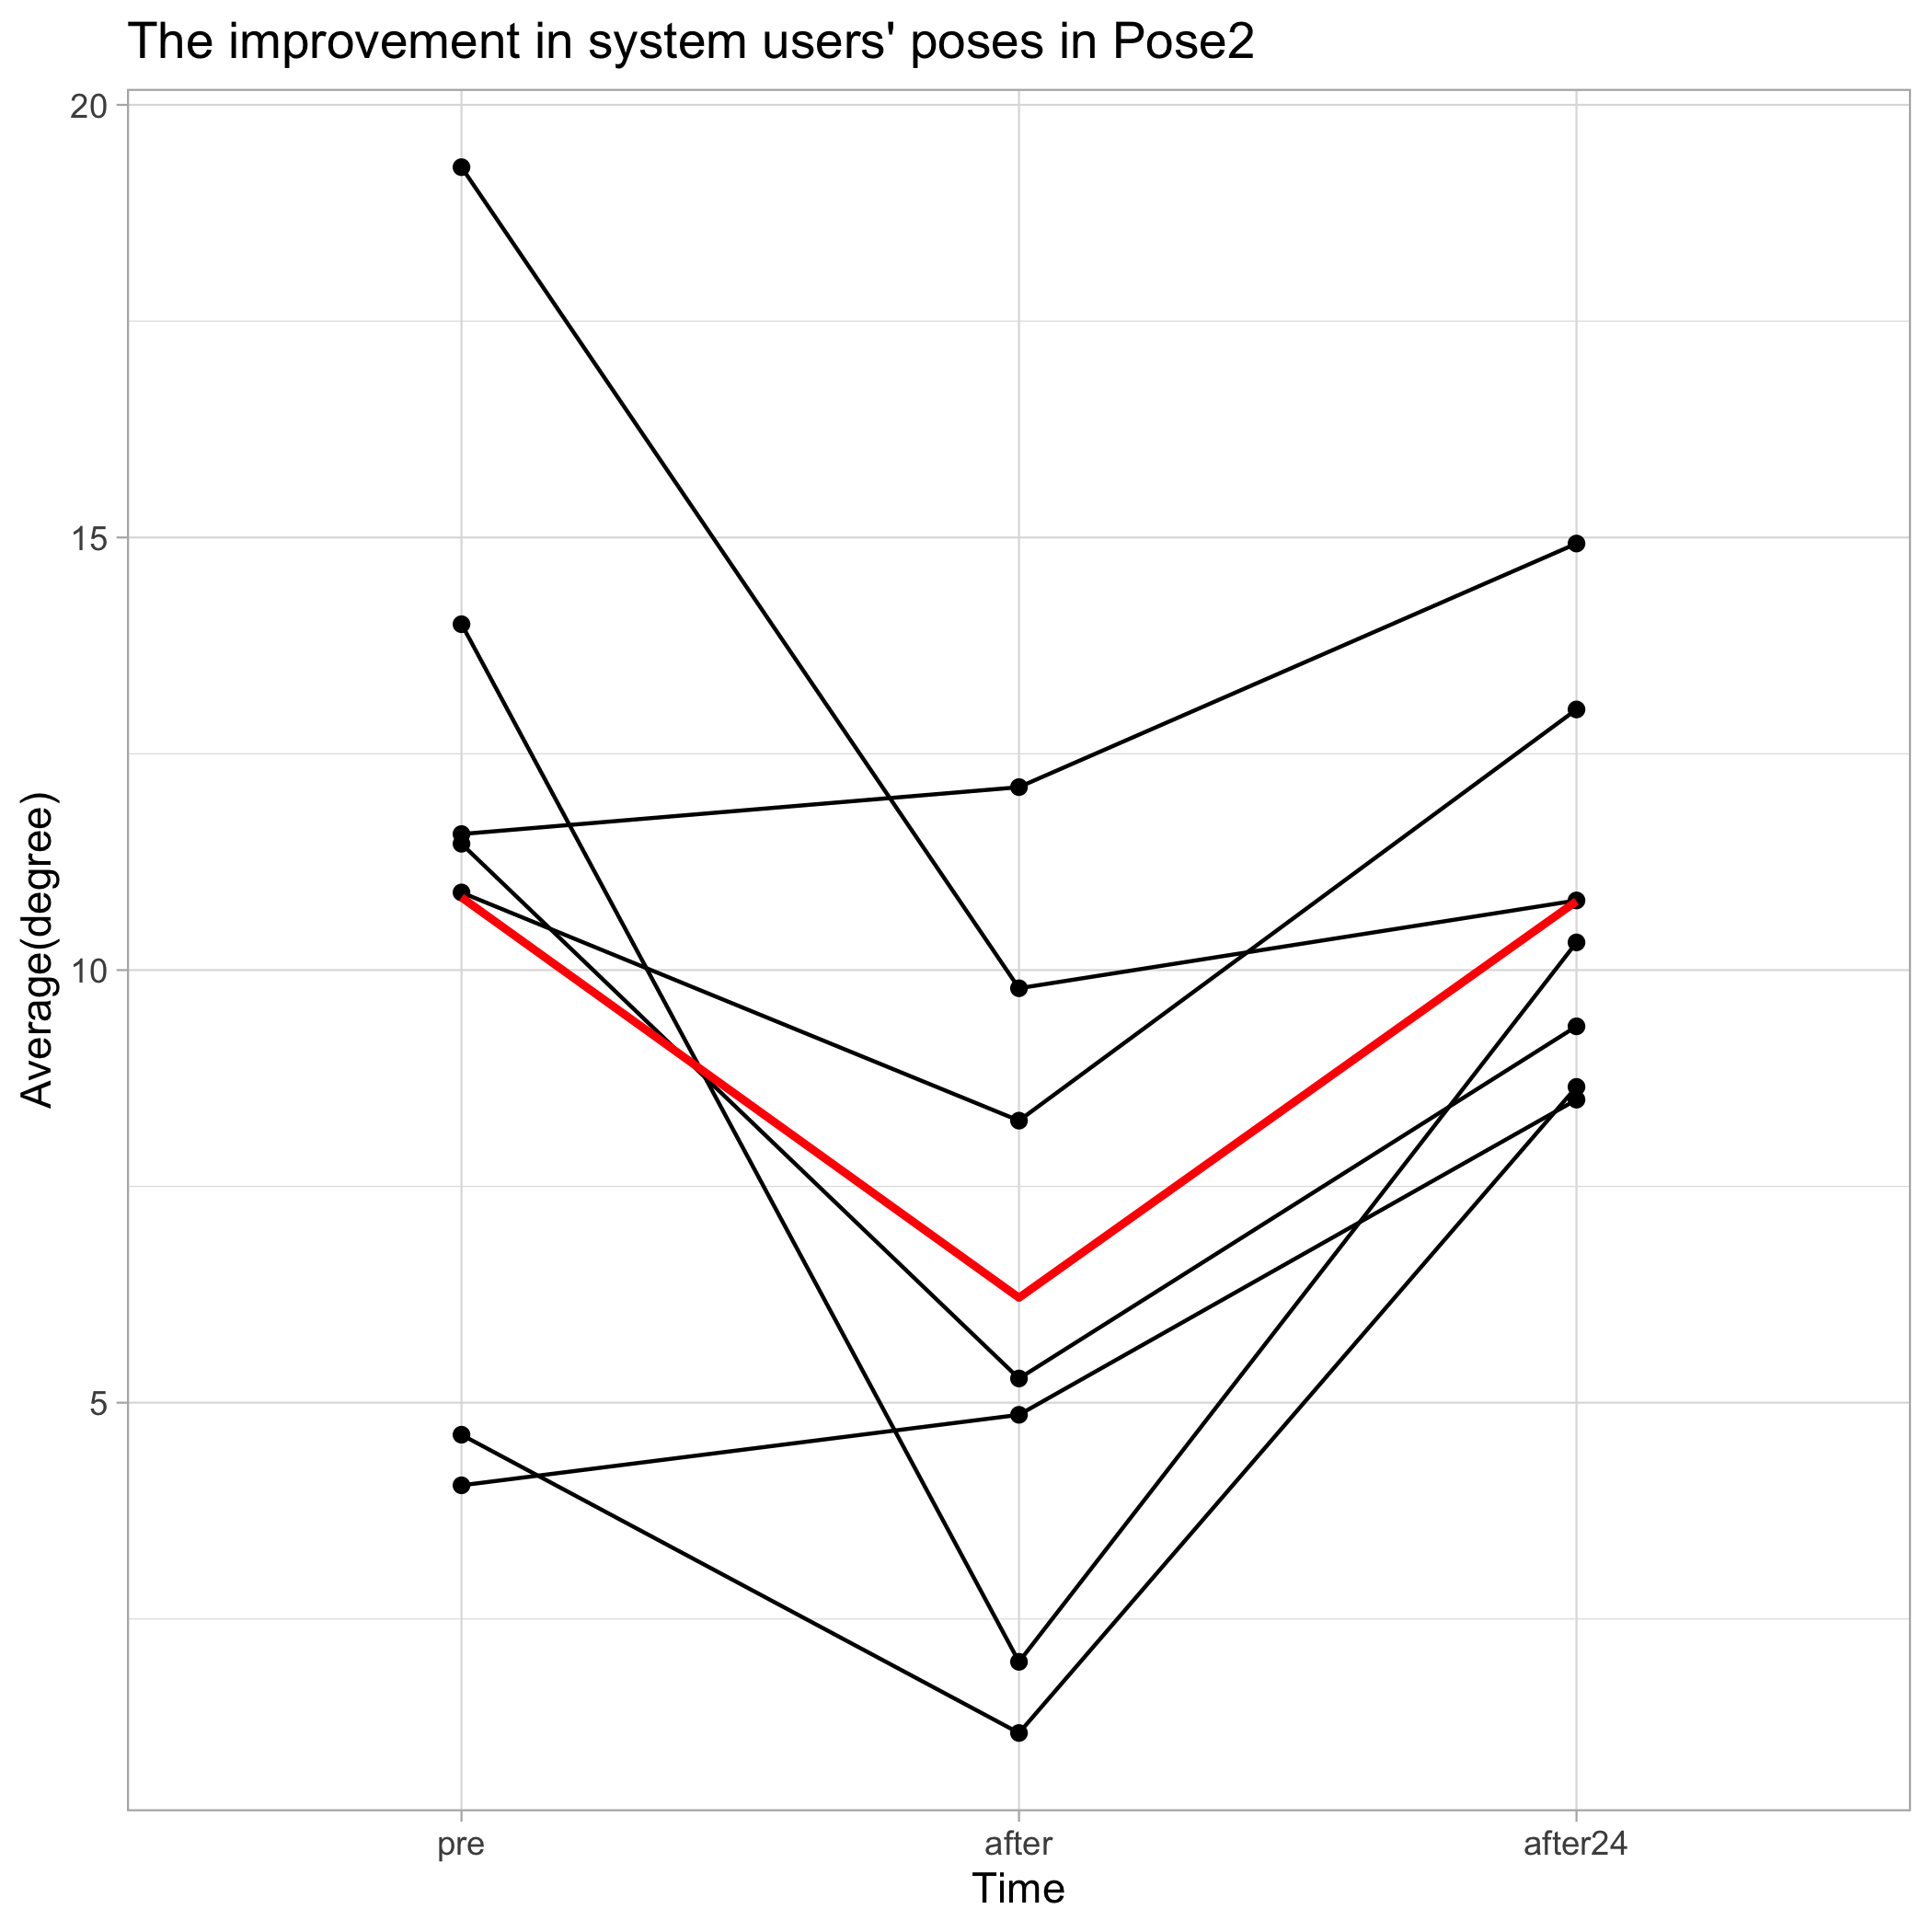
\includegraphics[width=9cm]{figures/pose2_system_true_graph.png}
        \caption{システム利用群のpose2の結果}
        \label{fig:pose2_system}
        \end{center}
      \end{figure}

      \begin{table}[ht]
        \centering
        \caption{pose2における練習後、練習から24時間後と練習前の比較}
        \begin{tabular}{lcr}
        \hline
        \textbf{比較対象} & \textbf{p-value} & \textbf{MD} \\ \hline
        after-pre & 0.07812 & -4.627143 \\ \hline
        after24-pre & 0.8125 & -0.04464286 \\ \hline
        \end{tabular}
        \label{table:pose2_system_p_value}
        \end{table}
    % ~~~~~~~~~~~~~~~~~~~~~~~~~~~~~~~~~~~~~~~~~~~~
    \subsubsection{鏡利用群の比較}
      図\ref{fig:pose1_mirror}にpose1に対して鏡を利用した群の練習前後、24時間後の結果と理想の角度との差の平均\(\bar{\theta}_{\text{angle\_dif}}\)を示す。


      7名のうち、5名の被験者が練習直後は練習前よりポーズが改善されていることがわかる。しかしながら、24時間後では練習前より改善されている被験者は4名であった。
      検定の結果では練習後と練習前の差は有意性を示すことができず(p=0.4688)、24時間後と練習前の差も統計的に有意性を示すことができなかった(p=0.5781)。表\ref{table:pose1_mirror_p_value}

      \begin{figure}[H]
        \begin{center}
        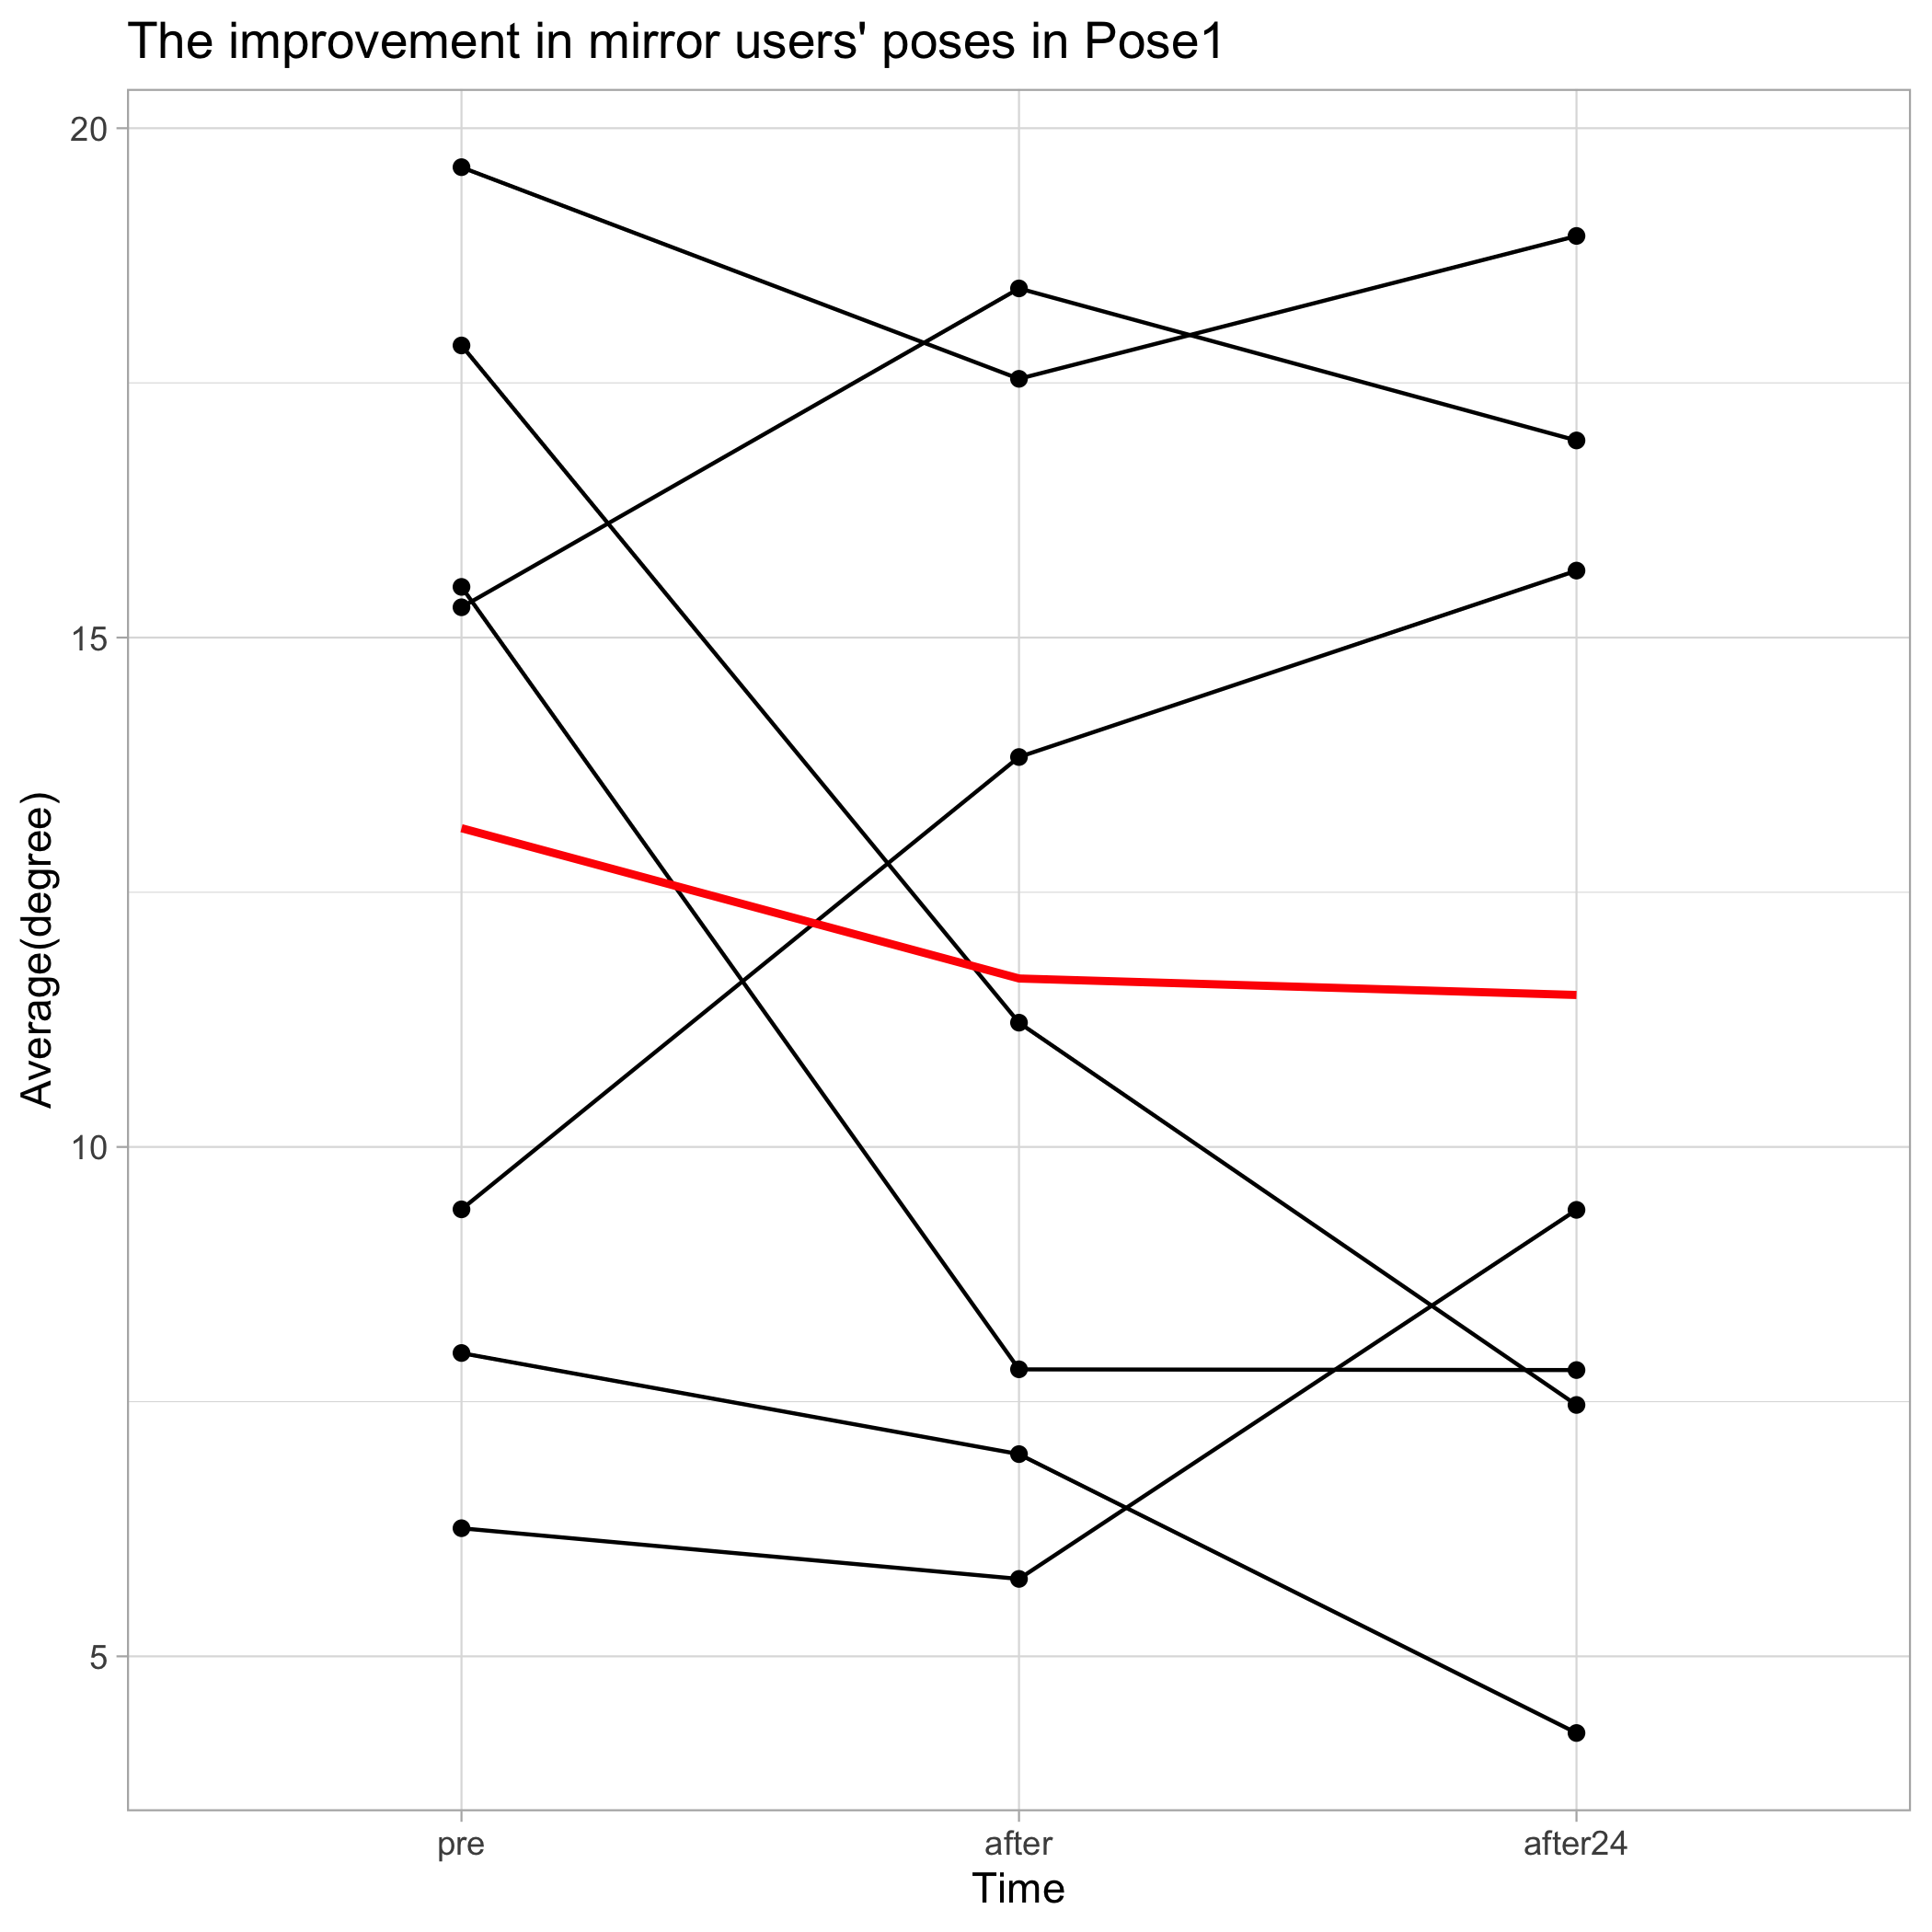
\includegraphics[width=9cm]{figures/pose1_system_false_graph.png}
        \caption{鏡利用群のpose1の結果}
        \label{fig:pose1_mirror}
        \end{center}
      \end{figure}

      \begin{table}[ht]
        \centering
        \caption{pose1における練習後、練習から24時間後と練習前の比較}
        \begin{tabular}{lcr}
        \hline
        \textbf{比較対象} & \textbf{p-value} & \textbf{MD} \\ \hline
        練習後-練習前 & 0.4688 & -1.475 \\ \hline
        24時間後-練習前 & 0.5781 & -1.637143 \\ \hline
        \end{tabular}
        \label{table:pose1_mirror_p_value}
        \end{table}

        図\ref{fig:pose2_mirror}にpose2に対して鏡を利用した群の練習前後、24時間後の結果と理想の角度との差の平均\(\bar{\theta}_{\text{angle\_dif}}\)を示す。


      7名のうち、6名の被験者が練習直後は練習前よりポーズが改善されていることがわかる。24時間後では練習前より改善されている被験者は3名であった。
      検定の結果では{\bf 練習後と練習前の差は有意であり、鏡の練習によって効果があったと考えられる(p=0.04688)}。 一方で、24時間後と練習前の差は統計的に有意性を示すことができなかった(p=0.8125)。表\ref{table:pose2_mirror_p_value}
      \begin{figure}[H]
        \begin{center}
        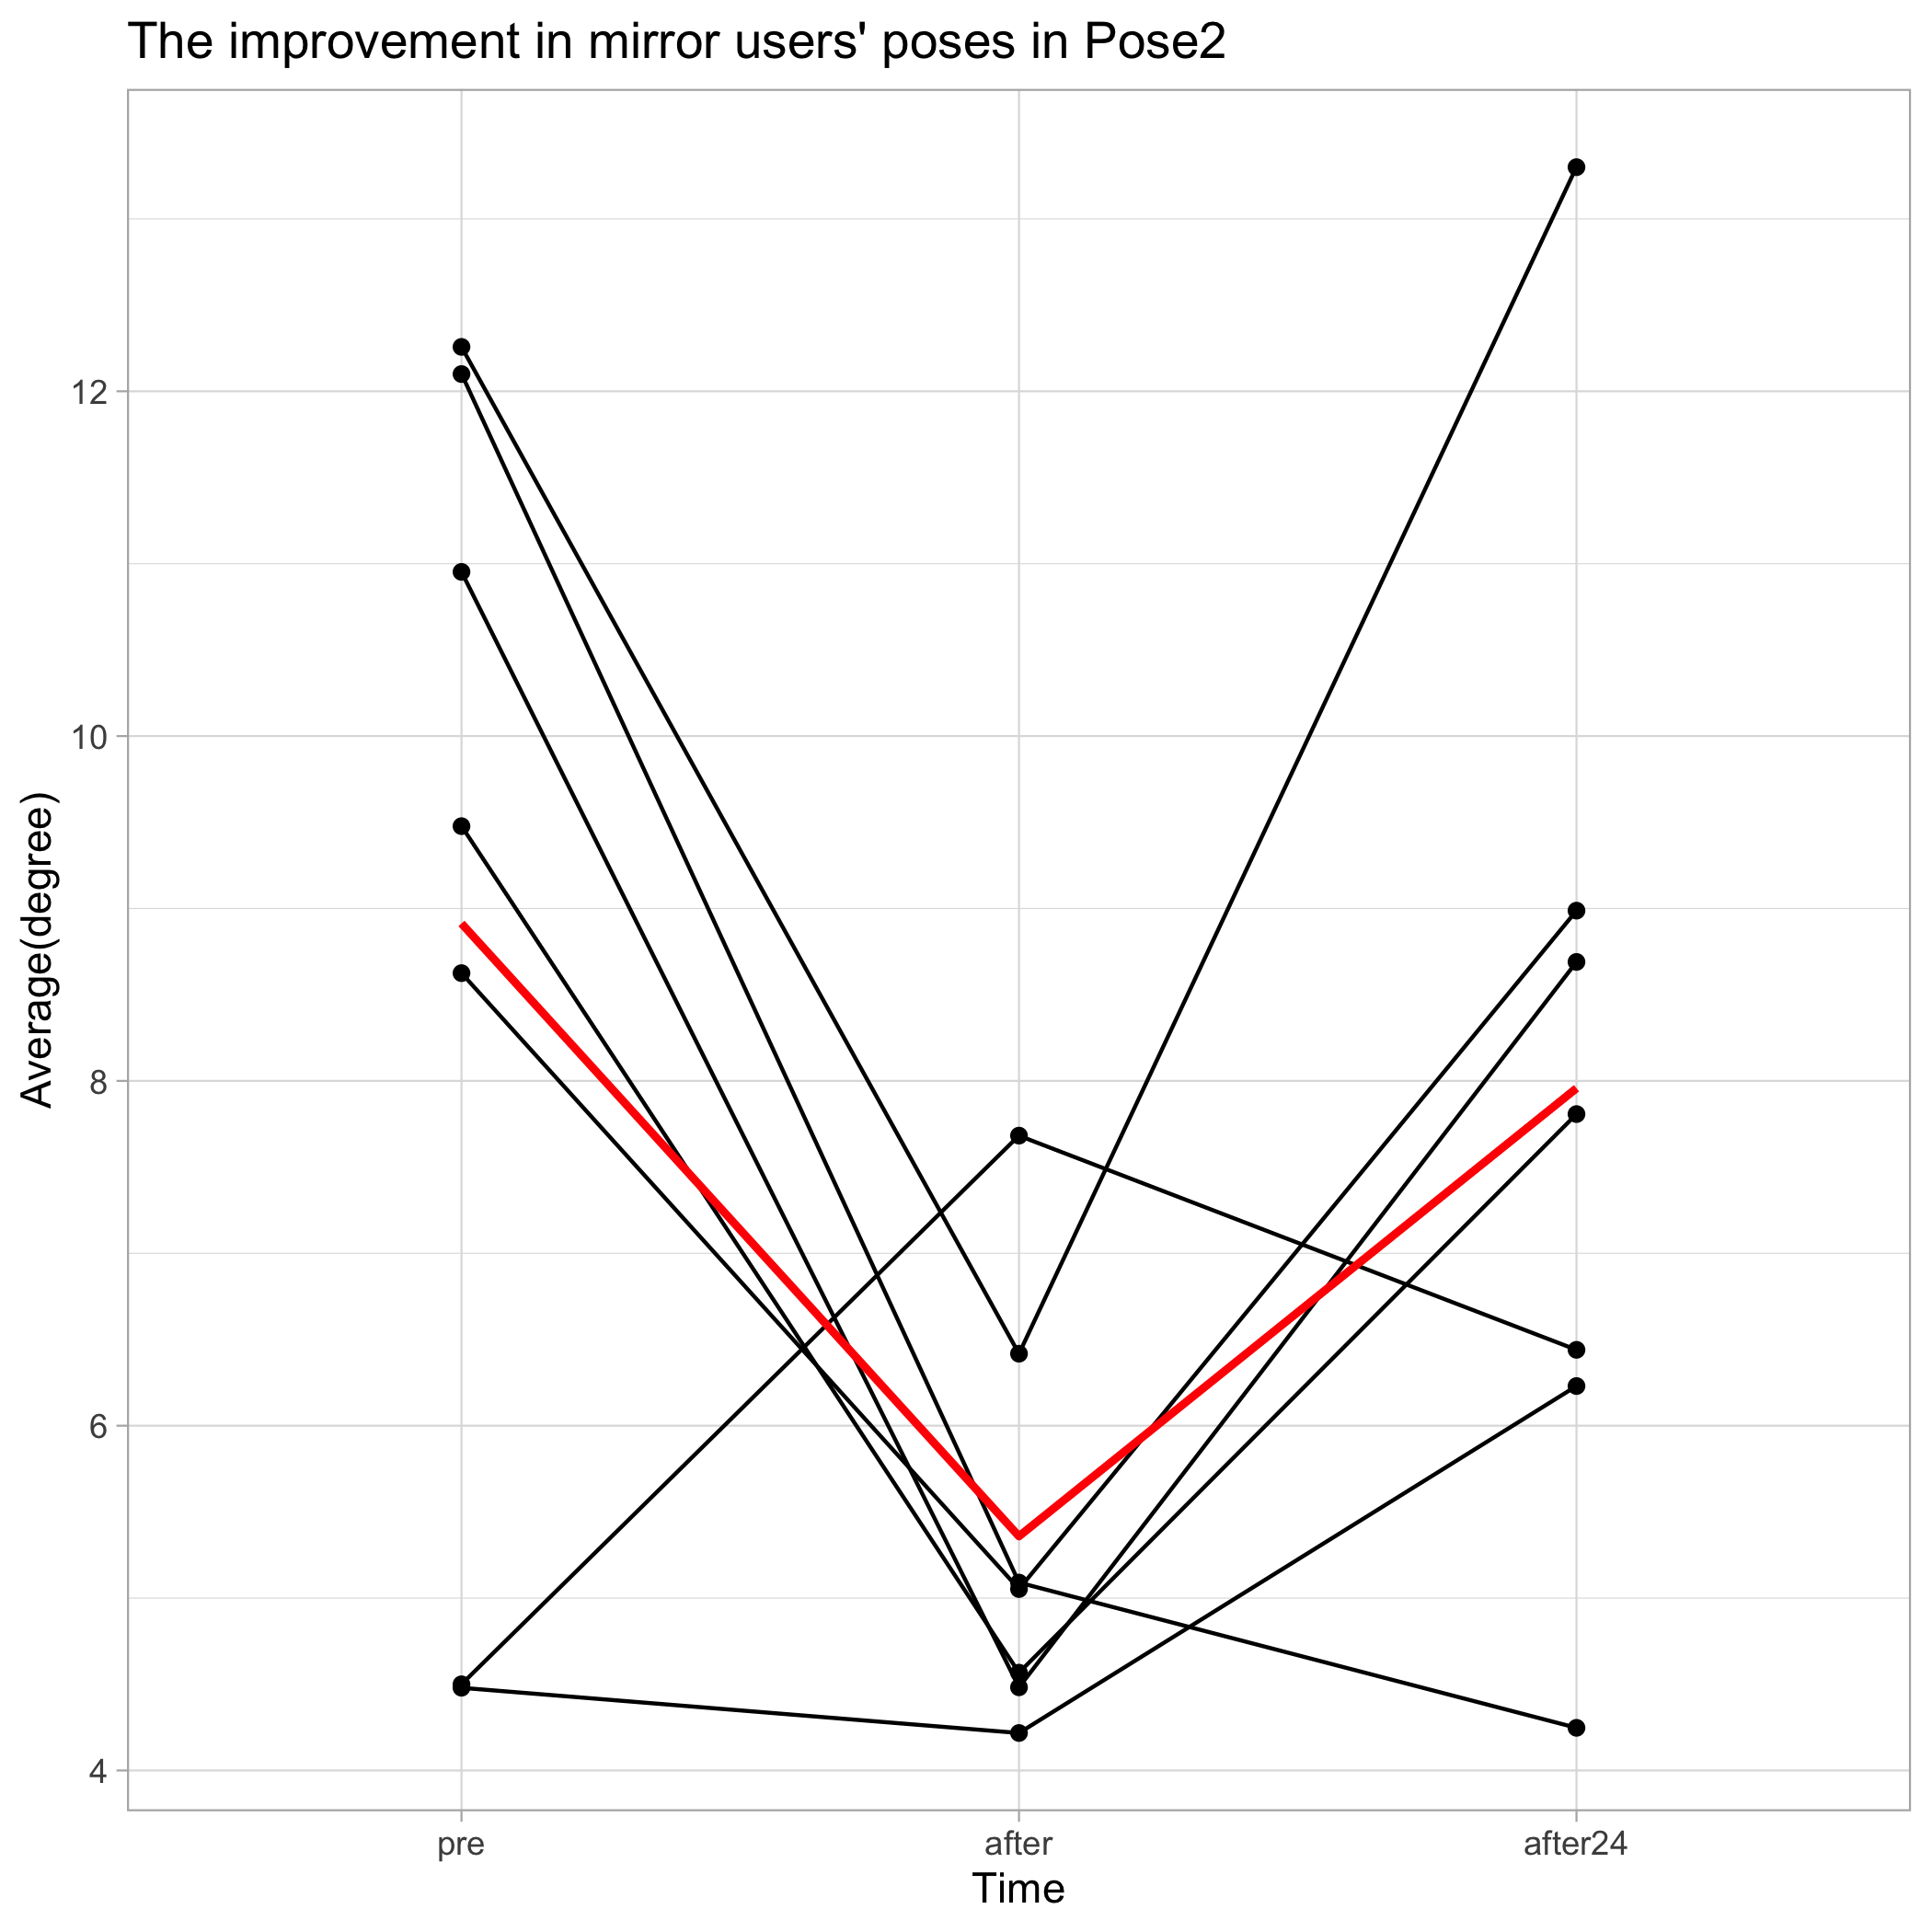
\includegraphics[width=9cm]{figures/pose2_system_false_graph.png}
        \caption{鏡利用群のpose2の結果}
        \label{fig:pose2_mirror}
        \end{center}
      \end{figure}

      \begin{table}[ht]
        \centering
        \caption{pose2における練習後、練習から24時間後と練習前の比較}
        \begin{tabular}{lcr}
        \hline
        \textbf{比較対象} & \textbf{p-value} & \textbf{MD} \\ \hline
        after-pre & 0.04688 & -3.554643 \\ \hline
        after24-pre & 0.8125 & -0.9557143 \\ \hline
        \end{tabular}
        \label{table:pose2_mirror_p_value}
        \end{table}

  \subsection{鏡利用群とシステム利用群の比較}
    ここでは同じポーズにおいてシステム利用群と鏡利用群の理想の角度との差の比較の結果を示す。

    \subsubsection{pose1における練習方法の違いによる比較}
      pose1に対してシステムを利用した群と鏡を利用した群の練習後の結果と理想の角度との差の平均\(\bar{\theta}_{\text{angle\_dif}}\)を図\ref{fig:pose1_after_practice}に、
      24時間後の比較を図\ref{fig:pose1_after24_practice}に示す。

      pose1においては、練習後の結果ではシステム利用群の方が鏡利用群よりもポーズが改善されていることがわかるが、p=0.7104と統計的に有意性を示すことができなかった。
      24時間後では表\ref{table:pose1_practice_p_value}にあるようにp=1と差を示すことができなかった。
      \begin{figure}[H]
        \begin{center}
        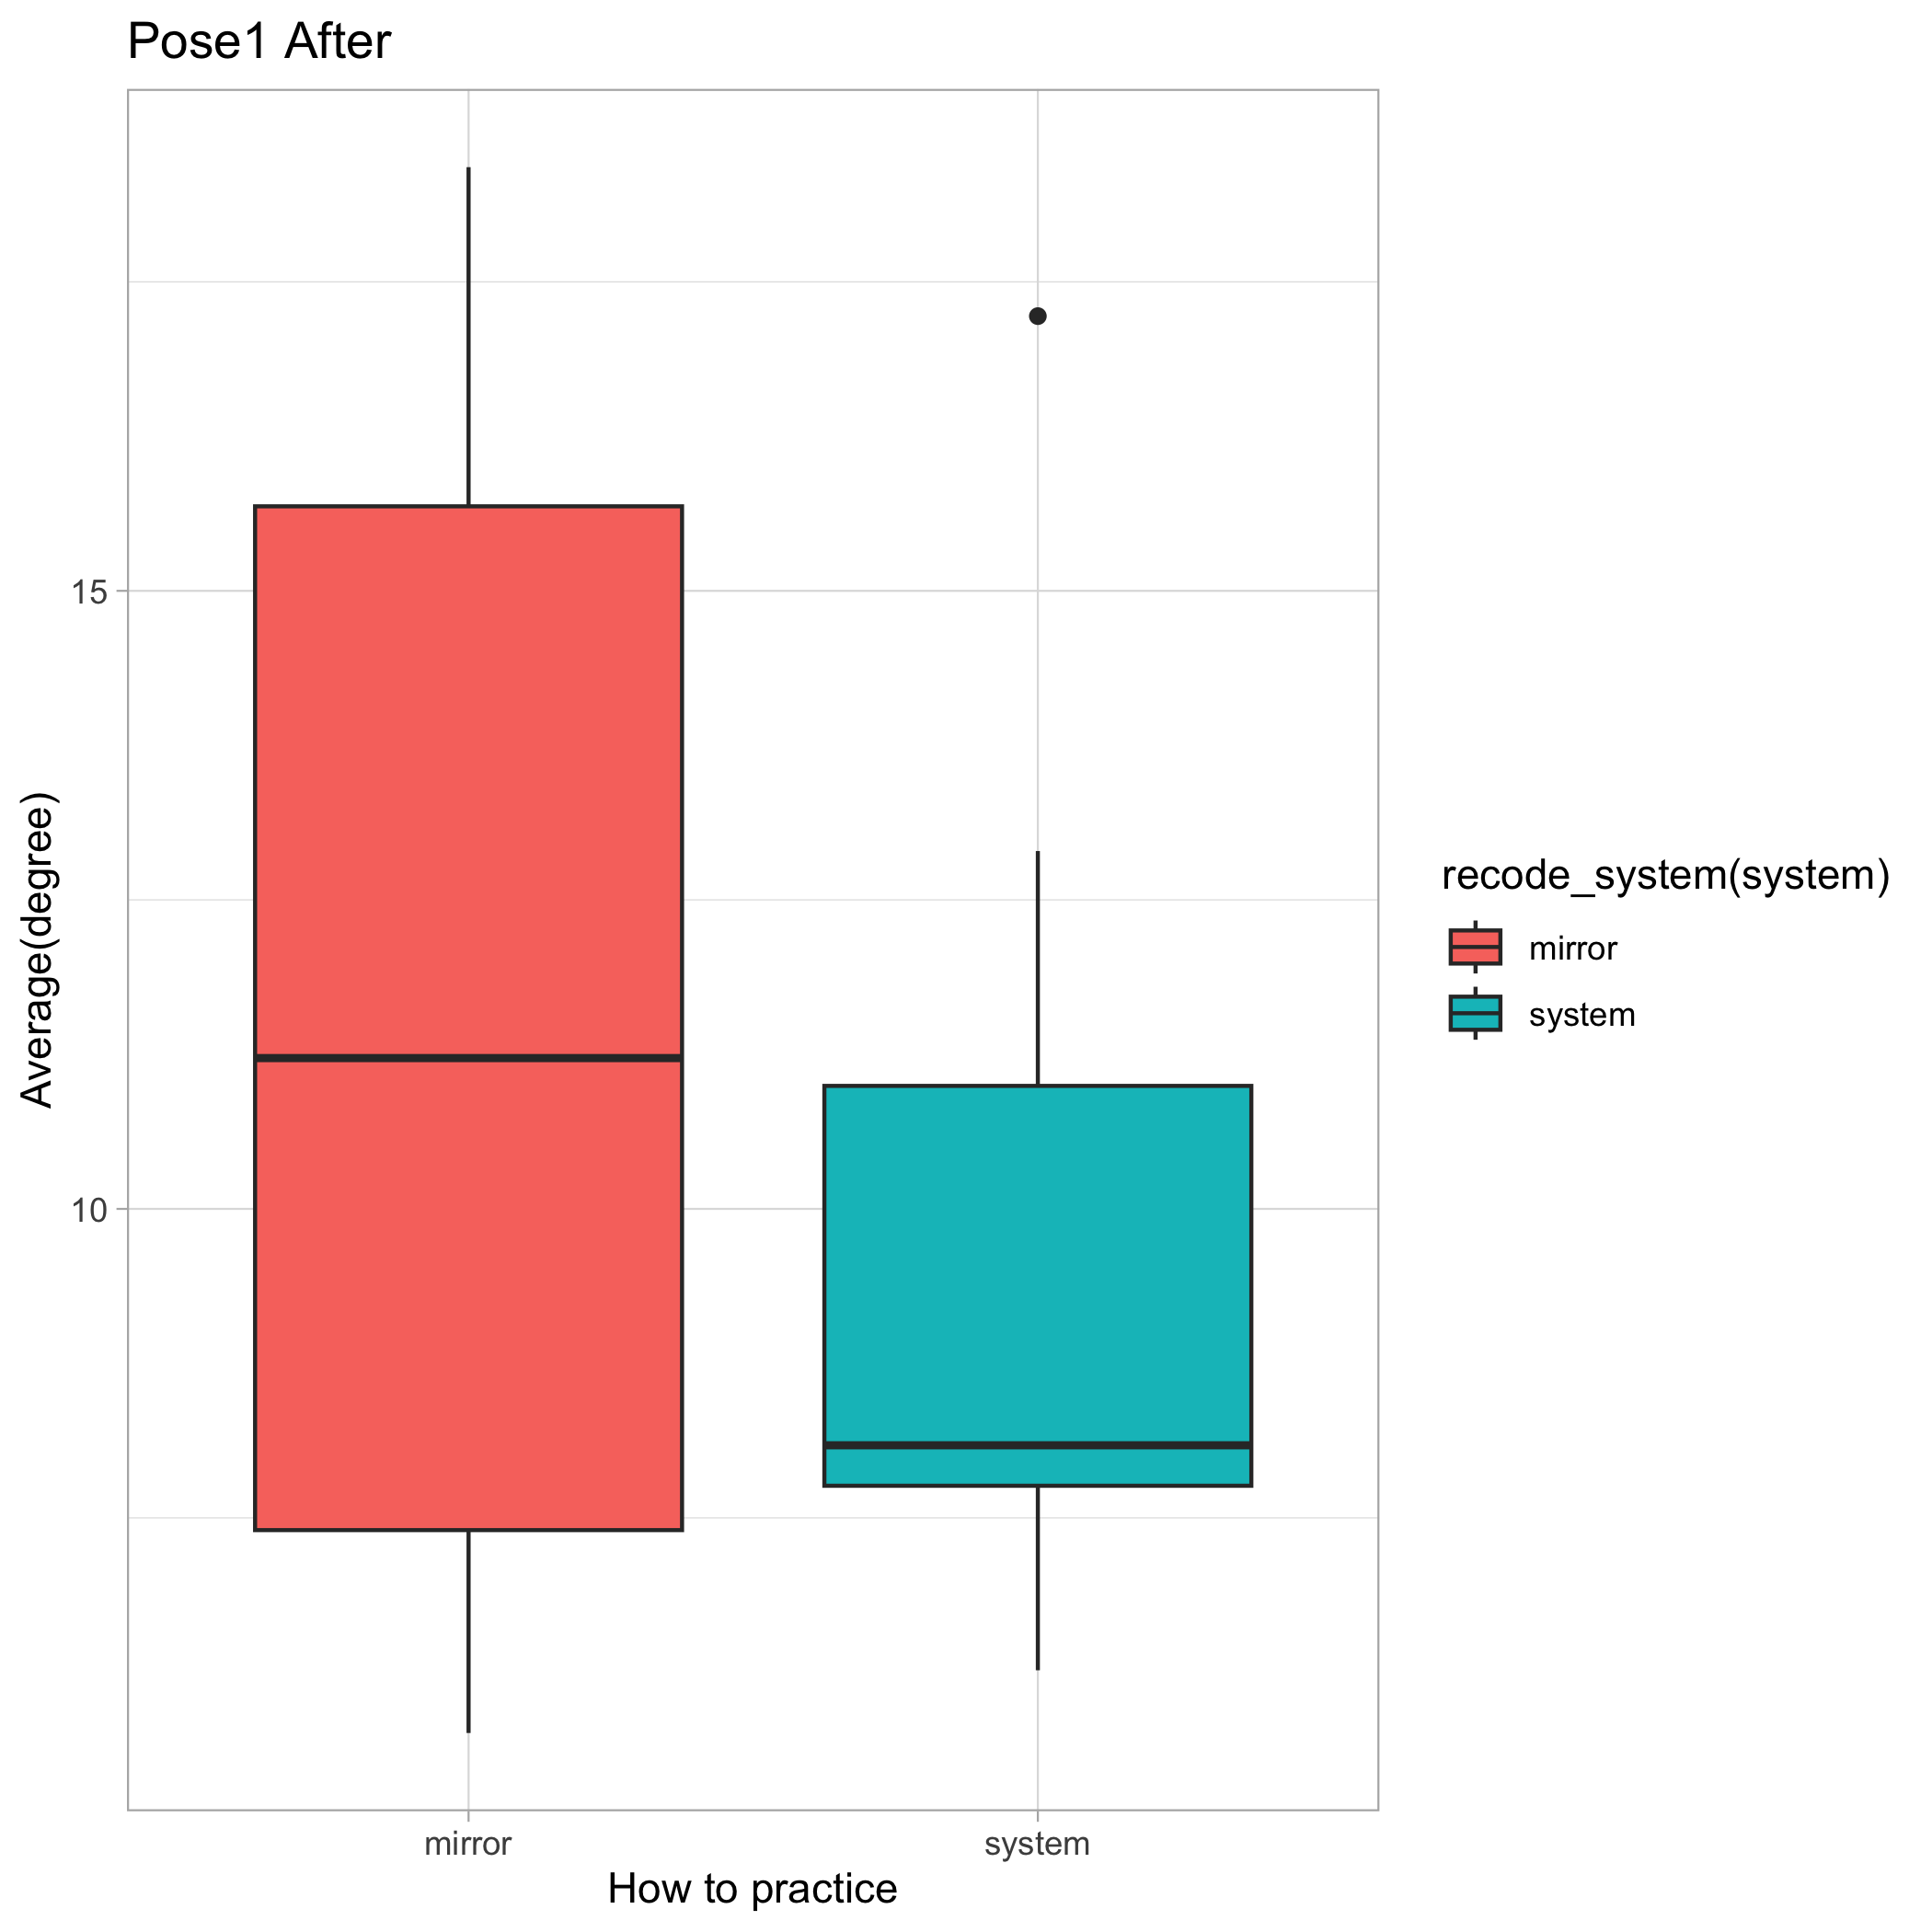
\includegraphics[width=9cm]{figures/pose1_after_boxplot.png}
        \caption{pose1における練習後の練習方法による比較}
        \label{fig:pose1_after_practice}
        \end{center}
      \end{figure}

      \begin{figure}[H]
        \begin{center}
        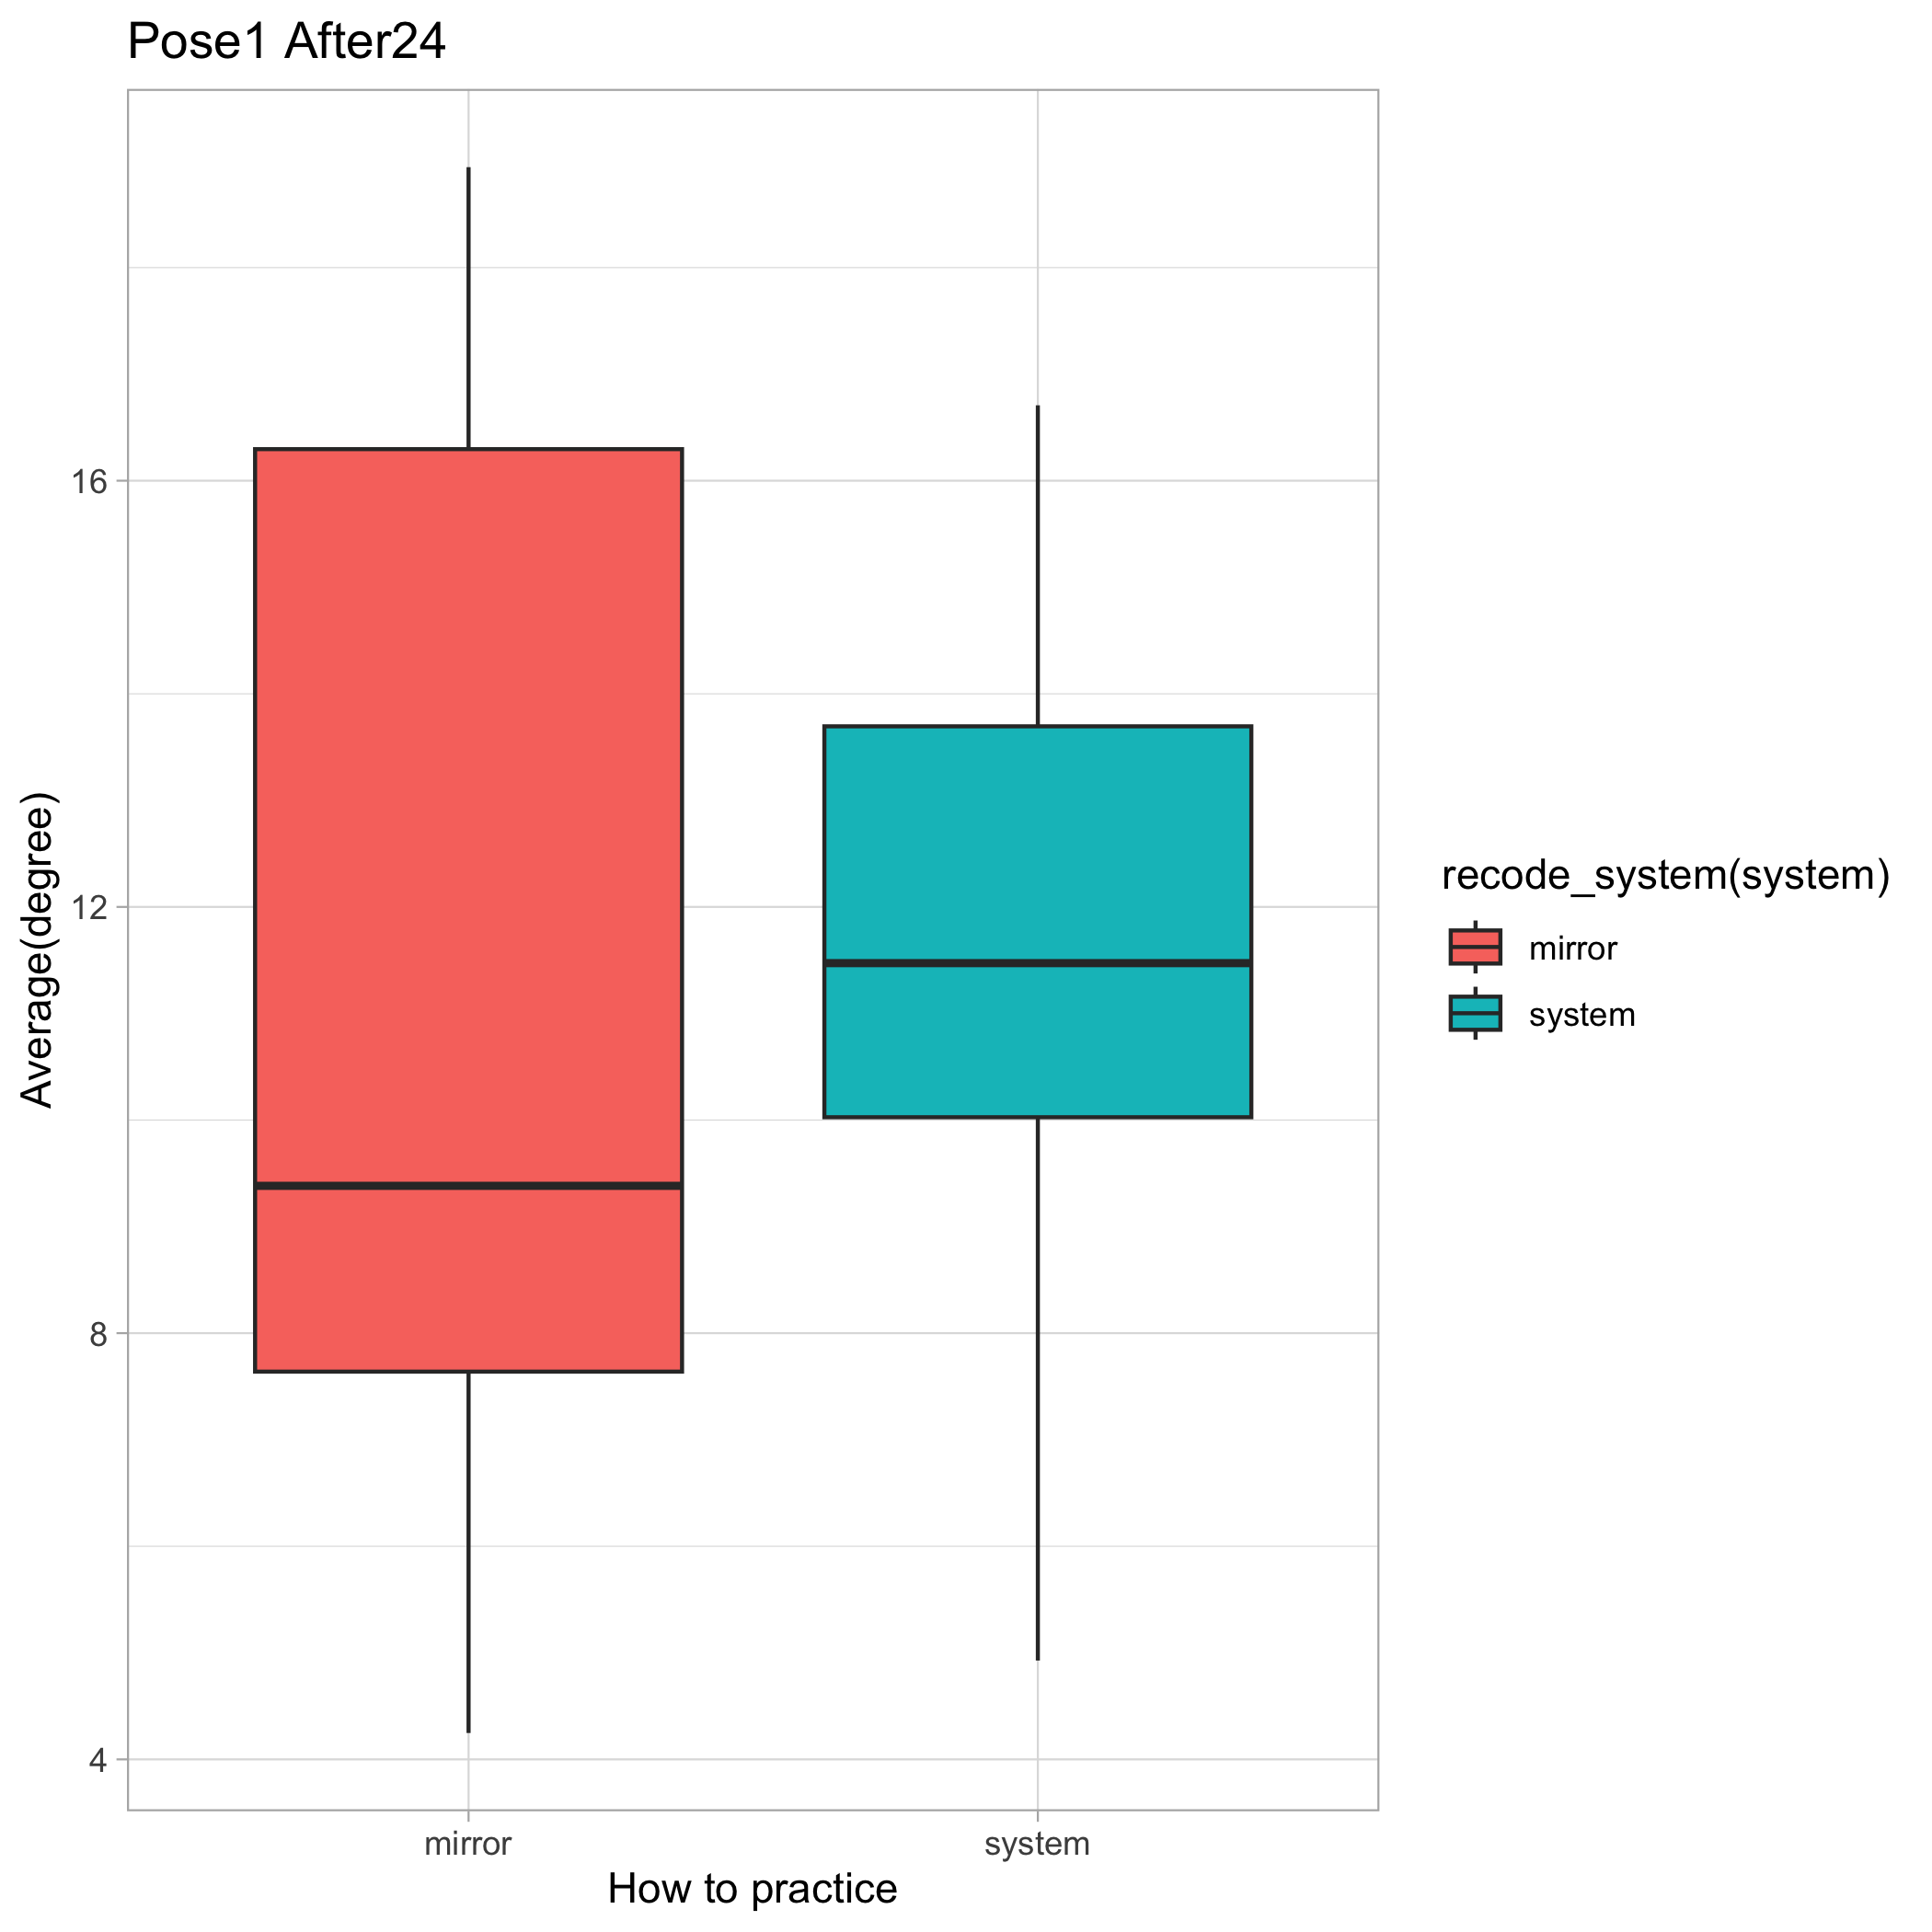
\includegraphics[width=9cm]{figures/pose1_after24_boxplot.png}
        \caption{pose1における24時間後の練習方法による比較}
        \label{fig:pose1_after24_practice}
        \end{center}
      \end{figure}

      \begin{table}[H]
        \centering
        \caption{pose1}
        \begin{tabular}{lcr}
        \hline
        \textbf{比較対象} & \textbf{p-value} & \textbf{平均差(システム-鏡)} \\ \hline
        after & 0.7104 & -1.784286\\ \hline
        after24 & 1 & 0.01535714\\ \hline
        \end{tabular}
        \label{table:pose1_practice_p_value}
        \end{table}
      
    \subsubsection{pose2における練習方法の違いによる比較}

      pose2に対してシステムを利用した群と鏡を利用した群の練習後の結果と理想の角度との差の平均\(\bar{\theta}_{\text{angle\_dif}}\)を図\ref{fig:pose2_after_practice}に、
      24時間後の比較を図\ref{fig:pose2_after24_practice}に示す。
      こちらでは表\ref{table:pose2_practice_p_value}に示すように統計的に有意とは言えないものの、pose1とは異なり練習後、24時間後ともに{\bf 鏡利用群の方が}システム利用群よりもポーズが改善されていることがわかる。
      \begin{figure}[H]
        \begin{center}
        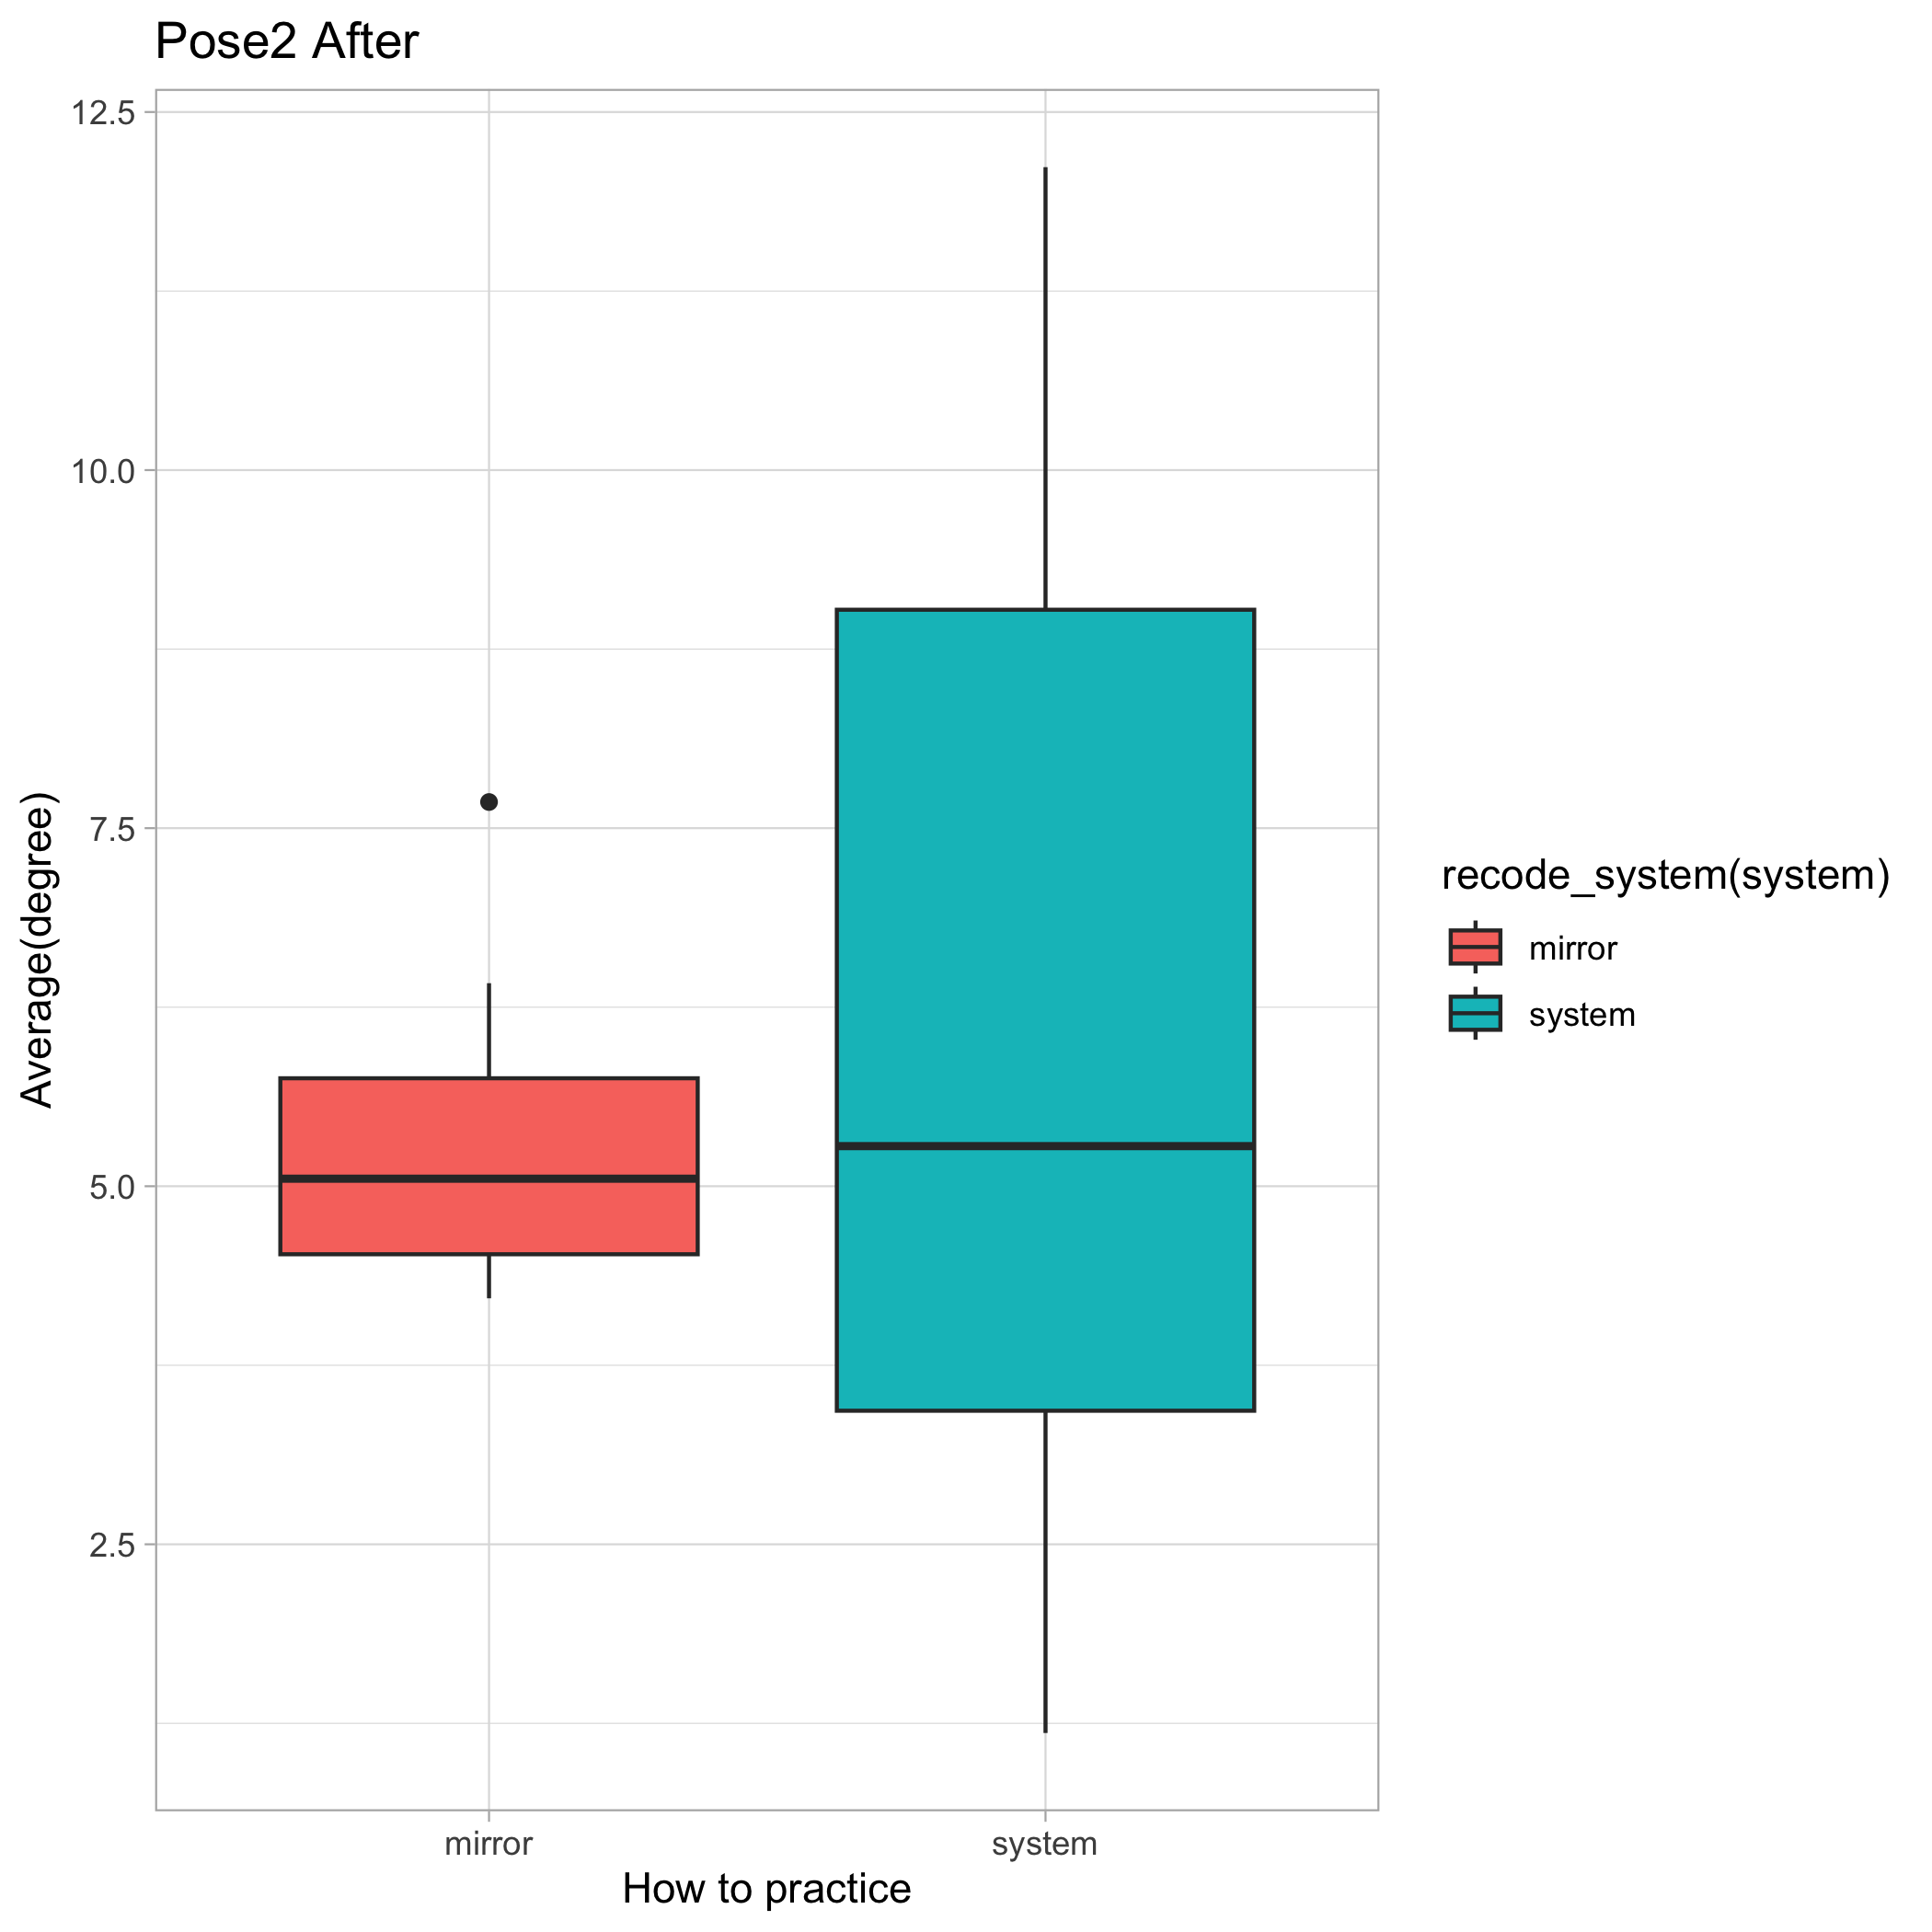
\includegraphics[width=9cm]{figures/pose2_after_boxplot.png}
        \caption{pose2における練習後の練習方法による比較}
        \label{fig:pose2_after_practice}
        \end{center}
      \end{figure}

      \begin{figure}[H]
        \begin{center}
        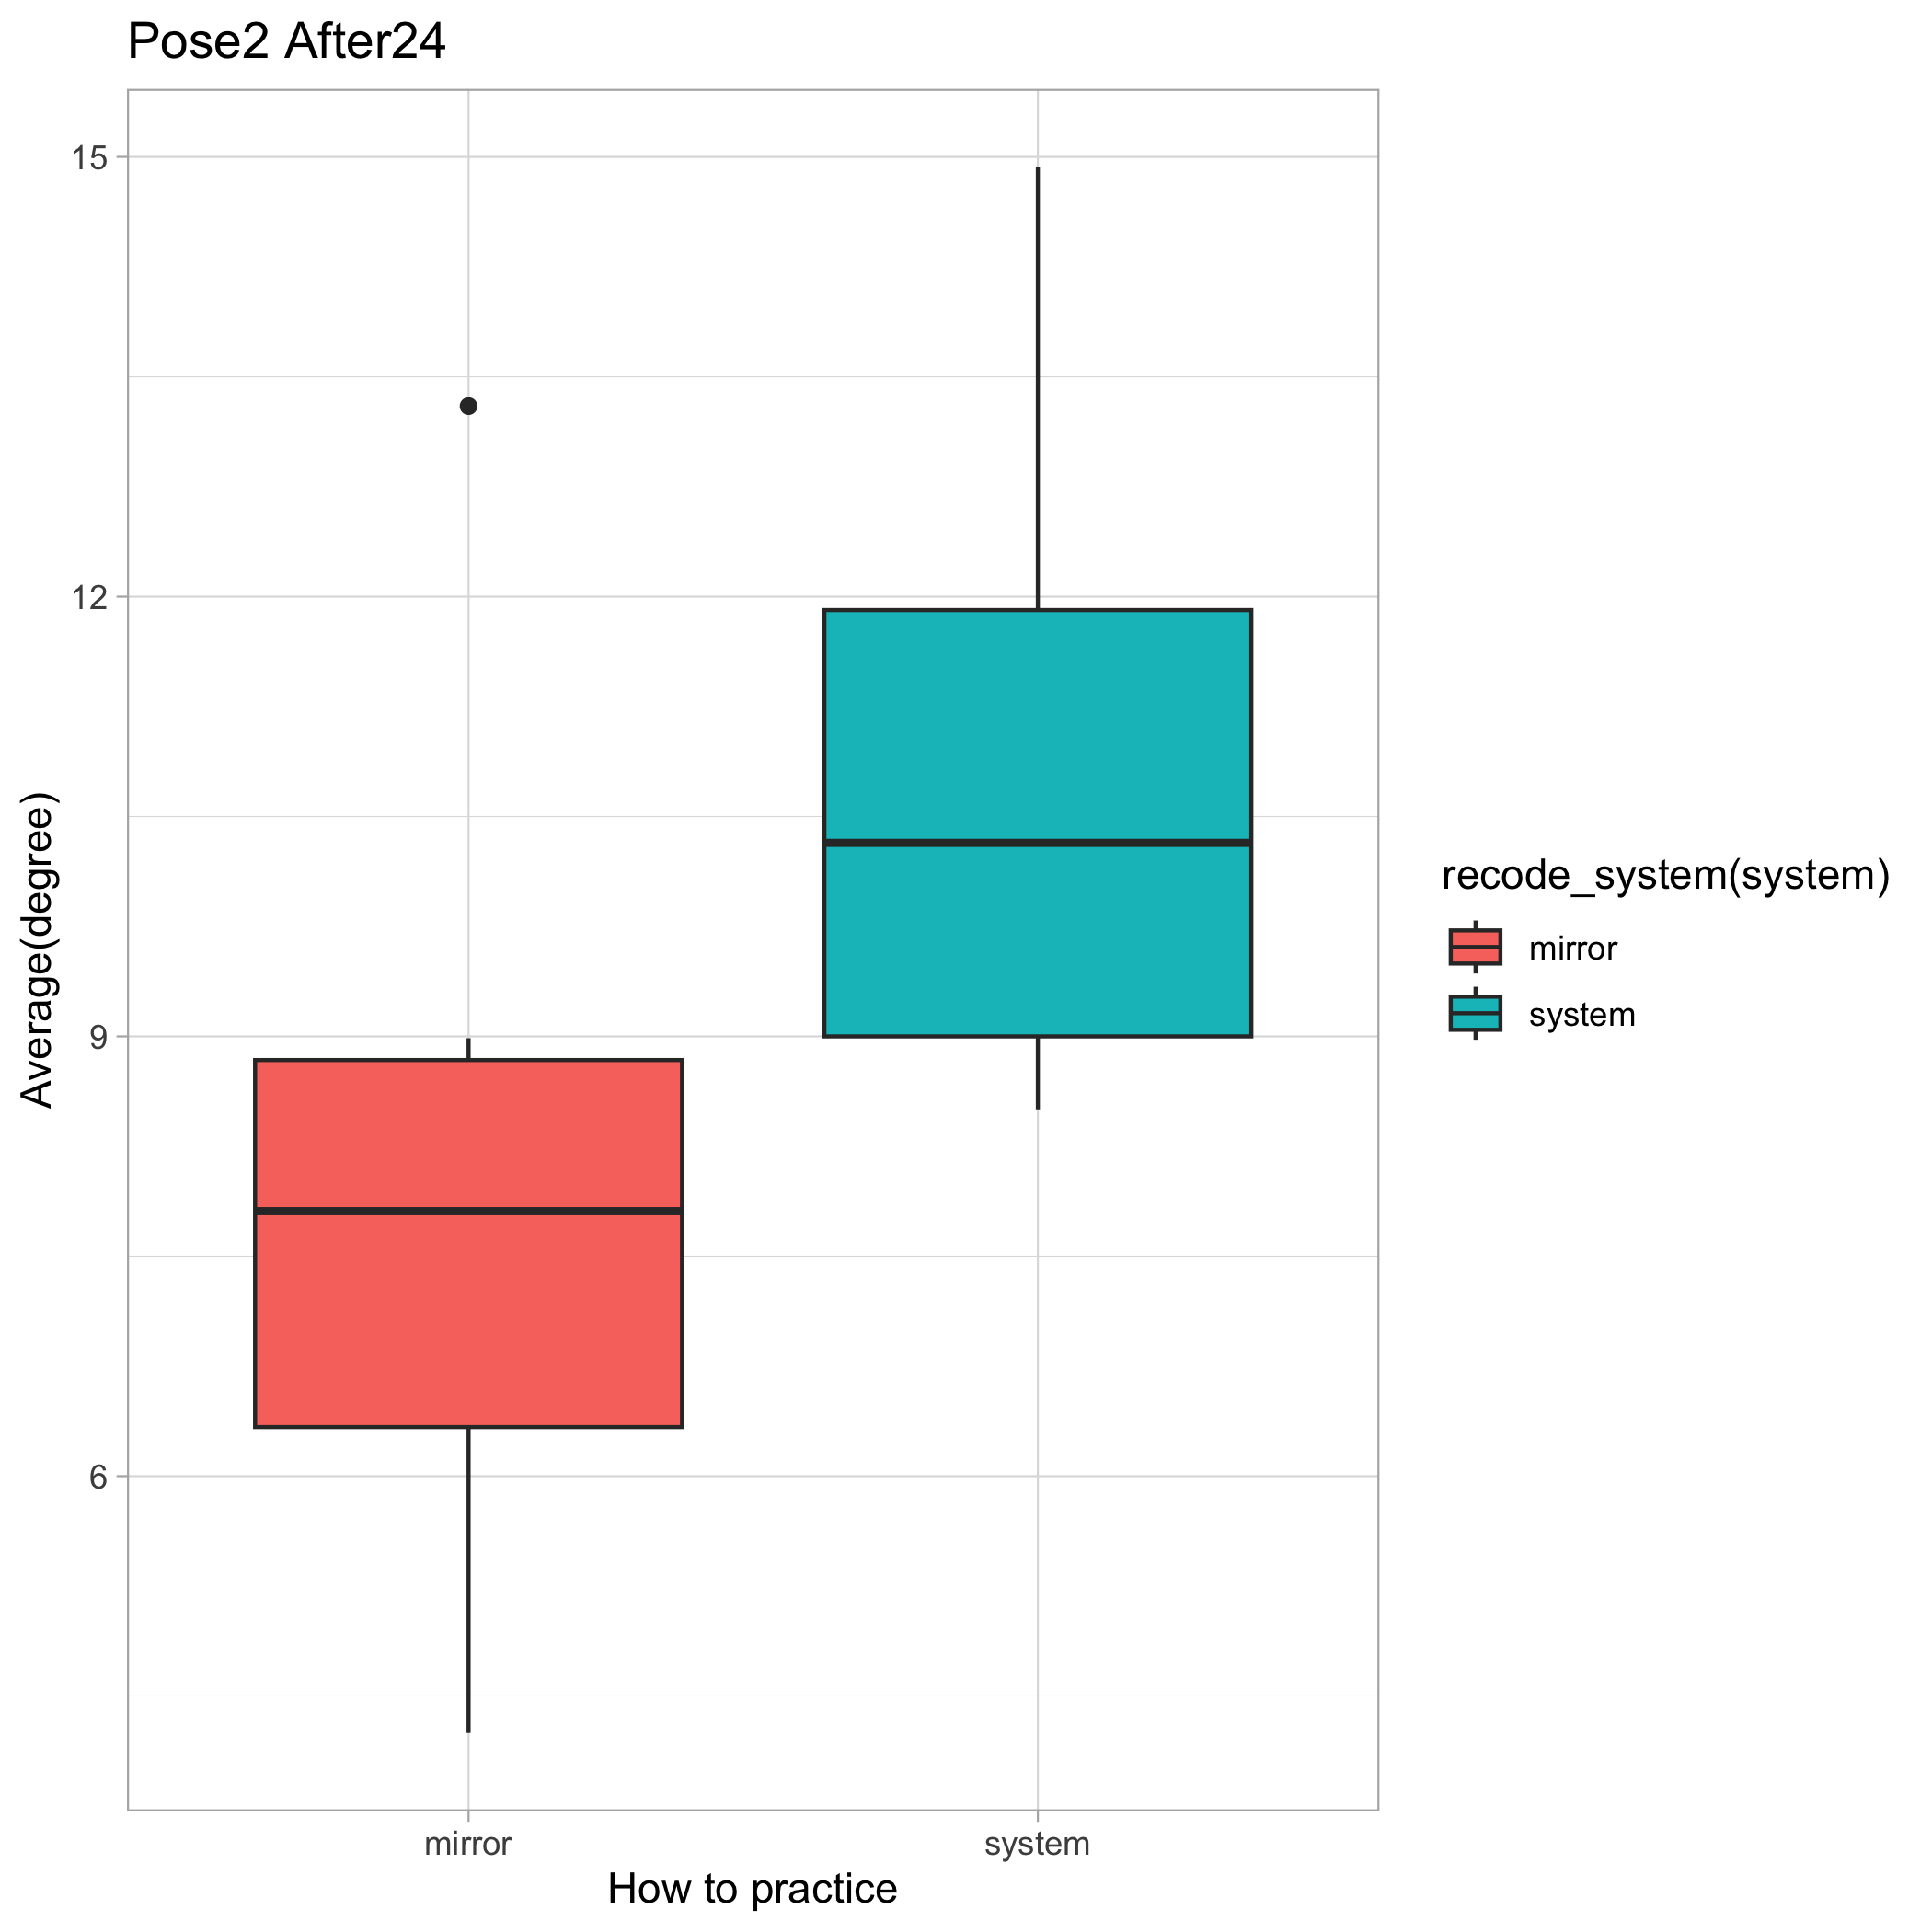
\includegraphics[width=9cm]{figures/pose2_after24_boxplot.png}
        \caption{pose2における24時間後の練習方法による比較}
        \label{fig:pose2_after24_practice}
        \end{center}
      \end{figure}

      \begin{table}[H]
        \centering
        \caption{pose2}
        \begin{tabular}{lcr}
        \hline
        \textbf{比較対象} & \textbf{p-value} & \textbf{平均差(システム-鏡)} \\ \hline
        after & 0.62 & 0.8546429 \\ \hline
        after24 & 0.07284 & 2.838214 \\ \hline
        \end{tabular}
        \label{table:pose2_practice_p_value}
        \end{table}


